\documentclass[aspectratio=169]{beamer}

\setbeamersize{text margin left=5mm, text margin right=5mm}

\defbeamertemplate{headline}{my header}{%
\vskip1pt%
\makebox[0pt][l]{\,\insertshortauthor}%
\hspace*{\fill}\insertshorttitle/\insertshortsubtitle\hspace*{\fill}%
\llap{\insertpagenumber/\insertpresentationendpage\,}
}
\setbeamertemplate{headline}[my header]

\let\olditem\item
\renewcommand{\item}{\setlength{\itemsep}{\fill}\olditem}

\usepackage{caption}
\usepackage{soul}
\usepackage{tkz-euclide}
\usetikzlibrary{calc}
\usepackage[]{algorithm2e}
\usepackage{changepage}
\usepackage{amssymb}
\usepackage{xcolor}
\usepackage{mathtools}
\usepackage{tcolorbox}
\usepackage{tikz}
\usepackage{tikz-3dplot}
\usepackage{tkz-euclide}
\usepackage{circuitikz}
\usepackage{mleftright}
\usetikzlibrary{arrows.meta, decorations.pathreplacing, positioning, shapes.geometric}

%% Fonts
\usefonttheme{professionalfonts}
\usefonttheme{serif}

\DeclareCaptionLabelFormat{blank}{}
\captionsetup[figure]{labelformat=blank}

%% Math definitions
\def\mf{\ensuremath\mathbf}
\def\mb{\ensuremath\mathbb}
\def\mc{\ensuremath\mathcal}
\def\lp{\ensuremath\left(}
\def\rp{\ensuremath\right)}
\def\lv{\ensuremath\left\lvert}
\def\rv{\ensuremath\right\rvert}
\def\lV{\ensuremath\left\lVert}
\def\rV{\ensuremath\right\rVert}
\def\lc{\ensuremath\left\{}
\def\rc{\ensuremath\right\}}
\def\ls{\ensuremath\left[}
\def\rs{\ensuremath\right]}
\def\bmx{\ensuremath\begin{bmatrix*}[r]}
\def\emx{\ensuremath\end{bmatrix*}}
\def\bmxc{\ensuremath\begin{bmatrix*}[c]}
\def\t{\lp t\rp}
\def\k{\ls k\rs}

\newcommand{\demoex}[2]{\onslide<#1->\begin{color}{black!60} #2 \end{color}}
\newcommand{\demoexc}[3]{\onslide<#1->\begin{color}{#2} #3 \end{color}}
\newcommand{\anim}[3]{\onslide<#1->{\begin{color}{#2!60} #3 \end{color}}}
\newcommand{\ct}[1]{\lp #1\rp}
\newcommand{\dt}[1]{\ls #1\rs}
\newcommand{\cols}[2]{\begin{columns}[#1] #2 \end{columns}}
\newcommand{\col}[2]{\begin{column}{#1} #2 \end{column}}

%% Mycolors
\definecolor{myred}{RGB}{192,0,0}
\definecolor{mygray}{RGB}{100,100,100}

%% Custom beamer color
\setbeamercolor{title}{fg=myred}
\setbeamercolor{subtitle}{fg=myred}
\setbeamerfont{title}{series=\bfseries}
% \setbeamercolor{frametitle}{bg=myred, fg=white}
\setbeamercolor{frametitle}{bg=mygray!10!, fg=myred}
\setbeamerfont{frametitle}{series=\bfseries}
\setbeamercolor{item}{fg=mygray}
\setbeamercolor{title in head/foot}{fg=myred}

% Move header to footer
\setbeamertemplate{headline}{}
\setbeamertemplate{footline}{
  \begin{beamercolorbox}[wd=\paperwidth,ht=2.25ex,dp=1ex,center]{footline}
    \inserttitle\hfill\insertauthor\hfill\insertdate\hfill\insertframenumber{}
  \end{beamercolorbox}
}

\title{Applied Linear Algebra in Data Analysis}

% A subtitle is optional and this may be deleted
\subtitle{Orthogonality}

\author{Sivakumar Balasubramanian}
% - Give the names in the same order as the appear in the paper.
% - Use the \inst{?} command only if the authors have different
%   affiliation.

\institute[Christian Medical College] % (optional, but mostly needed)
{
  \inst{}%
  Department of Bioengineering\\
  Christian Medical College, Bagayam\\
  Vellore 632002
}
% - Use the \inst command only if there are several affiliations.
% - Keep it simple, no one is interested in your street address.

\date{}
% - Either use conference name or its abbreviation.
% - Not really informative to the audience, more for people (including
%   yourself) who are reading the slides online

\subject{Lecture notes on linear systems}
% This is only inserted into the PDF information catalog. Can be left
% out. 

% If you have a file called "university-logo-filename.xxx", where xxx
% is a graphic format that can be processed by latex or pdflatex,
% resp., then you can add a logo as follows:

% \pgfdeclareimage[height=0.5cm]{university-logo}{university-logo-filename}
% \logo{\pgfuseimage{university-logo}}

% Delete this, if you do not want the table of contents to pop up at
% the beginning of each subsection:
\AtBeginSubsection[]
{
  \begin{frame}<beamer>{Outline}
    \tableofcontents[currentsection,currentsubsection]
  \end{frame}
}

% Let's get started
\begin{document}

\begin{frame}
  \titlepage
\end{frame}

% \begin{frame}[t]{References}
% \begin{itemize}
%     \item S Boyd, Applied Linear Algebra: Chapters 5.
%     \item G Strang, Linear Algebra: Chapters 3.
% \end{itemize}
% \end{frame}


\begin{frame}[t]{Orthogonality}
\begin{itemize}
\item Two vectors $\mf{x}, \mf{y} \in \mb{R}^n$ are orthogonal if $\mf{x}^\top\mf{y} = 0$.
\begin{center}
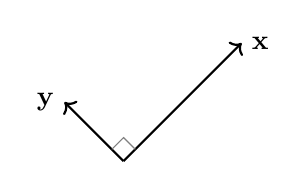
\begin{tikzpicture}[scale=0.75]
  \draw[black,thick,->] (0, 0) -- (2, 2) node[black, above, right]{$\mf{x}$};
  \draw[black,thick,->] (0, 0) -- (-1, 1) node[black, above, left]{$\mf{y}$};
  \draw [gray,thin](0.2,0.2) -- (0, 0.4) -- (-0.2, 0.2);
\end{tikzpicture}
\end{center}

\item The set of non-zero vectors, $V = \left\{\mf{v}_1, \mf{v}_2, \mf{v}_3, \ldots, \mf{v}_r\right\}$ is a set of mutually orthogonal vectors, if and only if,
\[ \mf{v}_i^\top\mf{v}_j = 0, \,\,\, 1 \leq i, j \leq r \text{ and } i \neq j \]

\item $V$ is also a linearly independent set of vectors. Why?

\end{itemize}
\end{frame}


\begin{frame}[t]{Orthogonality}
\begin{itemize}

\item If $\lV \mf{v}_i \rV = 1$, then $V$ is an \textbf{orthonormal} set of vectors.

\item A set of orthonormal vectors $V$ also form an \textbf{orthonormal basis} of the subsapce $span \left(V\right)$.

\end{itemize}
\end{frame}


\begin{frame}[t]{Orthogonal Subspaces}
\begin{itemize}
\item Two subspaces $\mc{V}, \mc{W} \subset \mb{R}^n$ are orthogonal if every vector in one subspace is orthogonal to every vector in the other subspace.
\[ \mf{v}^\top\mf{w} = 0, \,\,\, \forall \mf{v} \in \mc{V} \text{ and } \forall\mf{w} \in \mc{W} \implies \mc{V} \perp \mc{W} \]

\item If $\mc{V} + \mc{W} = \mb{R}^n$, and $\mc{V} \perp \mc{W}$, then $\mc{V}$ and $\mc{W}$ are \textbf{orthogonal complements} of each other.
\[ \mc{V}^{\perp} = \mc{W} \text{ or } \mc{W}^{\perp} = \mc{V}; \,\,\,\,\, \left(\mc{V}^{\perp}\right)^{\perp} = \mc{V} \]
\end{itemize}
\end{frame}


\begin{frame}[t]{Orthogonal Projection onto Subspaces}
\begin{columns}
\begin{column}{0.5\textwidth}
\begin{center}
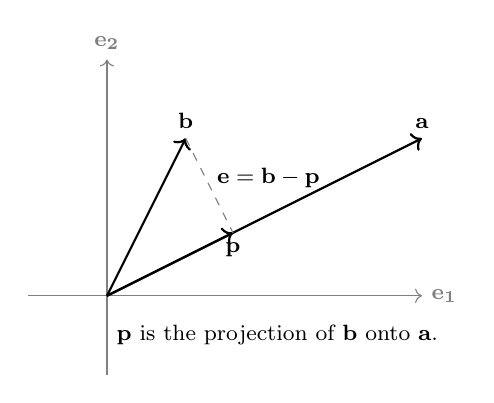
\begin{tikzpicture}[scale=1]
    \draw[gray, thin, ->] (-1, 0) -- (4, 0) node[right] {\footnotesize {$\mf{e_1}$}};
    \draw[gray, thin, ->] (0, -1) -- (0, 3) node[above] {\footnotesize {$\mf{e_2}$}};
    \draw[black, thick, ->] (0, 0) -- (4, 2) node[right, above] {\footnotesize {$\mf{a}$}};
    \draw[black, thick, ->] (0, 0) -- (1, 2) node[right, above] {\footnotesize {$\mf{b}$}};
    \draw[black, thick, ->] (0, 0) -- (1.6, 0.8) node[right, below] {\footnotesize{$\mf{p}$}};
    \draw[gray, thin, dashed] (1, 2) -- (1.6, 0.8) node[xshift=0.45cm, yshift=0.7cm, black] {{\footnotesize $\mf{e} = \mf{b - p}$}};
    \node[right, yshift=-0.5cm, black] at (0,0) {{\footnotesize $\mf{p}$ is the projection of $\mf{b}$ onto $\mf{a}$.}};
\end{tikzpicture}
\end{center}
% \vspace{-0.2cm}
\end{column}
\begin{column}{0.45\textwidth}
$\left\lVert \mf{e}\right\rVert$ is the distance of the point $\mf{b}$ from the line along $\mf{a}$. This distance is shortest when, $\mf{e} \perp \mf{a}$.
\[ \mf{a}^\top\left(\mf{b} - \mf{p}\right) = \mf{a}^\top\left(\mf{b} - \alpha \mf{a}\right) = \mf{a}^\top\mf{b} - \alpha \mf{a}^\top\mf{a} = 0 \]
\[ \alpha = \frac{\mf{a}^\top\mf{b}}{\mf{a}^\top\mf{a}} \implies \mf{p} = \frac{\mf{a}^\top\mf{b}}{\mf{a}^\top\mf{a}}\mf{a} \]
\[ \mf{p} = \frac{\mf{a}^\top\mf{b}}{\mf{a}^\top\mf{a}}\mf{a} =  \mf{a}\frac{\mf{a}^\top\mf{b}}{\mf{a}^\top\mf{a}} = \frac{\mf{a}\mf{a}^\top}{\mf{a}^\top\mf{a}}\mf{b} = \mf{Pb} \]
\end{column}
\end{columns}
\end{frame}


\begin{frame}[t]{Orthogonal Projection onto Subspaces}
\begin{itemize}
    \item We can project vectors onto high dimensional subspaces.
    \item Consider the subspace $\mc{S} \subseteq \mb{R}^n$ spanned by the orthonormal basis $\left\{\mf{u}_1, \mf{u}_2, \ldots \mf{u}_r\right\}$.\\

    \item We want to project a vector $\mf{b} \in\mb{R}^n$ onto $\mc{S}$ \\
    $\mf{b}_{\mc{S}}$ -- the orthogonal projection of $\mf{b}$ onto $\mc{S}$ is given by the following,
    \[ \mf{b}_{\mc{S}} = \mf{UU}^\top\mf{b}; \,\,\, \mf{U} = \begin{bmatrix}\mf{u}_1 & \mf{u}_2 & \ldots & \mf{u}_r \end{bmatrix} \]
    \[ \text{Projection matrix } \mf{P}_{\mc{S}} = \mf{UU}^\top \]
    \item A projection matrix is \textbf{idempotent}, i.e. $\mf{P}^2 = \mf{P}$. What does this mean in terms of projecting a vector on to a subspace?
\end{itemize}

\end{frame}


\begin{frame}[t]{Orthogonal Projection onto Subspaces}

\begin{itemize}
    \item Consider two matrices $\mf{U}_1, \mf{U}_2$ whose columns form an  orthonormal basis of the subspace $\mc{S} \subseteq \mb{R}^m $, $\mc{C}\lp\mf{U}_1\rp = \mc{C}\lp\mf{U}_2\rp$.

    \item The projection matrix onto the subspace $\mc{S}$, $\mf{U}_1\mf{U}_1^\top = \mf{U}_2\mf{U}_2^\top$. We get the same projection matrix irrespective of which orthonormal basis one uses.
\end{itemize}
\end{frame}


\begin{frame}[t]{Orthogonal Projection onto Subspaces}
\begin{itemize}
    \item Two subspaces $\mc{X}, \mc{Y} \subset \mb{R}^n$ are said to be \textbf{complementary subspaces} of $\mb{R}^n$, when
    \[ \mc{X} + \mc{Y} = \mb{R}^n \quad \text{and} \quad \mc{X}\cap\mc{Y} = \lc \mf{0} \rc \] 

    \item For complementary subspaces $\mc{X}, \mc{Y} \subset \mb{R}^n$, then any vector $\mf{v} \in \mb{R}^n$ can be uniquely represented as,
    \[ \mf{v} = \mf{v}_{\mc{X}} + \mf{v}_{\mc{Y}},  \,\,\ \mf{v}_\mc{X} \in \mc{X}, \,\, \mf{v}_\mc{Y} \in \mc{Y} \] 

    $\mf{v}_\mc{X}, \mf{v}_\mc{Y}$ are the components of $\mf{v}$ in $\mc{X}$ and $\mc{Y}$, respectively.

    \item When $\mc{X} \perp \mc{Y}$, then $\mf{v}_\mc{X}^\top\mf{v}_\mc{Y} = 0$; $\mf{v}_\mc{X}, \mf{v}_\mc{Y}$ are orthogonal components. 
\end{itemize}
\end{frame}


\begin{frame}[t]{Relationship between the Four Fundamental Subspaces of $\mf{A}$}
\begin{itemize}
    \item $\mc{C}\lp\mf{A}\rp, \mc{N}\lp\mf{A}^\top\rp \subseteq \mb{R}^n$ are orthogonal complements.
    \[ \mc{C}\lp\mf{A}\rp \perp \mc{N}\lp\mf{A}^\top\rp \implies \mc{C}\lp\mf{A}\rp + \mc{N}\lp\mf{A}^\top\rp = \mb{R}^n \]

    \item $\mc{C}\lp\mf{A}^\top\rp, \mc{N}\lp\mf{A}\rp \subseteq \mb{R}^m$ are orthogonal complements.
    \[ \mc{C}\lp\mf{A}^\top\rp \perp \mc{N}\lp\mf{A}\rp \implies \mc{C}\lp\mf{A}^\top\rp + \mc{N}\lp\mf{A}\rp = \mb{R}^m  \]
\end{itemize}
\end{frame}


\begin{frame}[t]{Orthogonal Projection onto Subspaces}
\vspace{-0.2cm}
\begin{itemize}
    \item An orthogonal projection matrix $\mf{P}_\mc{S}$ onto a subspace $\mc{S}$ represents a linear mapping, $\mf{P}_\mc{S}: \mb{R}^n \to \mb{R}^n$. What are the four fundamental subspaces of $\mf{P}_\mc{S}$?\\
    \[ \mc{C}\lp \mf{P}_\mc{S}\rp = \mc{S}; \quad \mc{N}\lp \mf{P}_\mc{S}\rp = \mc{S}^\perp \]
    \[ \mc{N}\lp \mf{P}_\mc{S}^\top\rp = \mc{S}^\perp; \quad \mc{C}\lp \mf{P}_\mc{S}^\top\rp = \mc{S} \]
\end{itemize}
\end{frame}


\begin{frame}[t]{Relationship between the Four Fundamental Spaces}
\vspace{-0.25cm}
\begin{columns}
\begin{column}{0.6\textwidth}
\begin{center}
\begin{circuitikz}[scale=0.6]
    \filldraw[fill=black] (0,0) circle (0.1cm);
    \draw[thick,rotate around={30:(0,0)}] (0,0) rectangle (3,4);
    \draw[thick,rotate around={30:(0,0)}] (0,0) rectangle (-1.5,-2);
    \node[yshift=0.1cm, xshift=-0.3cm] at (0, 0) {$\mf{0}$};
    \node[yshift=2.2cm] at (0, 0) {$\mc{C}\lp\mf{A}^\top\rp$};
    \node[yshift=-1.9cm] at (0, 0) {$\mc{N}\lp\mf{A}\rp$};
    \draw[thick,rotate around={-30:(10,0)}] (10,0) rectangle (6,5);
    \draw[thick,rotate around={-30:(10,0)}] (10,0) rectangle (13,-3.75);
    \node[yshift=0.1cm, xshift=0.3cm] at (10, 0) {$\mf{0}$};
    \node[yshift=2.5cm] at (10, 0) {$\mc{C}\lp\mf{A}\rp$};
    \node[yshift=-1.9cm] at (10, 0) {$\mc{N}\lp\mf{A}^\top\rp$};
    
    \draw[blue, thin, dashed] (-0.5, 3) to node[currarrow] {} (10,2);
    \draw[red, thin, dashed] (-0.5, 3) -- (1.9, 0.6);
    \filldraw[fill=black] (-0.5,3) circle (0.1cm);
    \node[yshift=-0.3cm] at (-0.5,3) {$\mf{x}_r$};
    \draw[blue, thin, dashed] (-0.2,-1.5) to node[currarrow] {} (10,0);
    \draw[red, thin, dashed] (-0.2,-1.5) -- (1.9, 0.6);
    \filldraw[fill=black] (-0.2,-1.5) circle (0.1cm);
    \node[yshift=-0.25cm] at (-0.2,-1.5) {$\mf{x}_n$};
    \filldraw[fill=black] (10,0) circle (0.1cm);

    \draw[blue, thin, dashed] (1.9,0.6) to node[currarrow] {} (10,2);
    \filldraw[fill=black] (1.9,0.6) circle (0.1cm);
    \node[right, yshift=-0.3cm] at (1.9,0.6) {$\mf{x} = \mf{x}_r + \mf{x}_n$};
    
    \filldraw[fill=black] (10,2) circle (0.1cm);
    \node[yshift=-0.3cm] at (10,2) {$\mf{b}$};
\end{circuitikz}
\end{center}
\end{column}

\begin{column}{0.4\textwidth}
\begin{footnotesize}
\begin{itemize}
    \item $\mf{x}_r$ and $\mf{x}_n$ are the components of $\mf{x} \in \mb{R}^m$ in the row space and nullspace of $\mf{A}$.
    \item \textbf{Nullspace} $\mc{N}\lp\mf{A}\rp$ is mapped to $\mf{0}$.
    \[ \mf{A}\mf{x}_n = \mf{0} \]
    \item \textbf{Row space} $\mc{C}\lp\mf{A}^\top\rp$ is mapped to the \textbf{column space} $\mc{C}\lp\mf{A}\rp$.
    \[ \mf{A}\mf{x}_r = \mf{A}\lp\mf{x}_r + \mf{x}_n\rp = \mf{Ax} = \mf{b} \]
    \item The mapping from the \textbf{row space} to the \textbf{column space} is invertible, i.e. every $\mf{x}_r$ is mapped to a unique element in $\mc{C}\lp\mf{A}\rp$
    \item What sort of mapping does $\mf{A}^\top$ do?
\end{itemize}
\end{footnotesize}
\end{column}
\end{columns}
\end{frame}


\begin{frame}[t]{Gram-Schmidt Orthogonalization}
\vspace{-0.25cm}
\begin{itemize}
    \item Given a linearly independent set of vectors $\mc{B} = \left\{\mf{x}_1, \mf{x}_2, \ldots \mf{x}_n\right\}$, where $\mf{x}_i \in \mb{R}^m, \,\,\, \forall i \in \left\{1, 2, \ldots n\right\}$, how can we find a orthonormal basis $\left\{\mf{u}_1, \mf{u}_2, \ldots \mf{u}_n\right\}$ for $span\lp \mc{B}\rp $? $\longrightarrow$ \textbf{Gram-Schmidt Algorithm}
    \item Its an iterative procedure that can also detect if a given set $\mc{B}$ is linearly dependent.
\end{itemize}
\begin{small}
\begin{center}
\fbox{\begin{minipage}{35em}
\begin{algorithm}[H]
  \KwData{$\left\{\mf{x}_i\right\}_{i=1}^n$}
  \KwResult{Return an orthonormal basis $\left\{\mf{u}_i\right\}_{i=1}^{n}$ if the set $\mc{B}$ is linearly independent, else return nothing.}
  \For{$i = 1, 2, \ldots n$}{
  1. $\tilde{\mf{q}}_i = \mf{x}_i - \sum_{j=1}^{i-1}\lp \mf{u}_j^\top\mf{x}_i\rp \mf{u}_i$ $\longrightarrow$(\textbf{Orthogonalization step})\;
  2. \textbf{If} $\tilde{\mf{q}}_i=0$ \textbf{then} \textbf{return}\;
  3. $\mf{u}_i = \tilde{\mf{q}}_i / \left\Vert\tilde{\mf{q}}_i\right\Vert $ $\longrightarrow$(\textbf{Normalization step})\;
  }
  \textbf{return} $\left\{\mf{u}_i\right\}_{i=1}^n$\;
\end{algorithm}
\end{minipage}}
\end{center}
\end{small}
\end{frame}


\begin{frame}[t]{Gram-Schmidt Orthogonalization}
\vspace{-0.25cm}
\begin{itemize}
    \item The algorithm can also be conveniently represented in a matrix form.
    \[ \mc{B} = \left\{\mf{a}_1, \mf{a}_2, \ldots \mf{a}_n\right\} \]
    \[ \text{Let } \mf{U}_1 = 0_{m \times 1}\,\,\,\text{ and }\,\,\,\mf{U}_i = \begin{bmatrix*}[r]\mf{u}_1 & \mf{u}_2 & \ldots & \mf{u}_{i-1}\end{bmatrix*} \in \mb{R}^{m \times (i - 1)}
    \]
    \[ \mf{U}_i^\top\mf{x}_i = \begin{bmatrix*}[c]\mf{u}_1^\top\mf{x}_i\\\mf{u}_2^\top\mf{x}_i\\\vdots\\\mf{u}_{i-1}^\top\mf{x}_i\\\end{bmatrix*}\,\,\,\text{ and }\,\,\, \mf{U}_i\mf{U}_i^\top\mf{x}_i = \sum_{j=1}^{i-1}\lp \mf{u}_j^\top\mf{x}_i\rp \mf{u}_j
    \]
    \[ \mf{u}_i = \frac{\lp \mf{I} - \mf{U}_i\mf{U}_i^\top\rp \mf{x}_i}{\left\lVert \lp \mf{I} - \mf{U}_i\mf{U}_i^\top\rp \mf{x}_i\right\rVert} \]
\end{itemize}
\end{frame}

\begin{frame}[t]{$\mf{QR}$ Decomposition}
\vspace{-0.25cm}
\begin{footnotesize}
\begin{itemize}
    \item Gram-Schmidt procedure leads us to another form of matrix  decomposition -- \textbf{QR decomposition}.
    \item Given a matrix $\mf{A} = \begin{bmatrix*}\mf{a}_1&\mf{a}_2&\ldots&\mf{a}_n\end{bmatrix*} \in \mb{R}^{n \times n}$, whose columns form a linearly independent set.\\
    Gramm-Schmidt algorithm produces a orthonormal basis $\left\{\mf{q}_1, \mf{q}_2, \ldots \mf{q}_n\right\}$ for $\mc{C}\lp \mf{A}\rp $.
    \[ \mf{q}_1 = \frac{\mf{a}_1}{r_1}\,\,\,\text{ and }\,\,\, \mf{q}_i = \frac{\mf{a}_i - \sum_{j=1}^{i-1}(\mf{q}_j^\top\mf{a}_i)\mf{q}_j}{r_k} \]
    where, $r_1 = \left\lVert \mf{a}_1\right\rVert$ and $r_k = \left\lVert \mf{a}_i - \sum_{j=1}^{i-1}(\mf{q}_j^\top\mf{a}_i)\mf{q}_j\right\rVert$.
    \[ \mf{a}_1 = r_1\mf{q}_1\,\,\,\text{ and }\,\,\,\mf{a}_i = r_i\mf{q}_i + \sum_{j=1}^{i-1}\lp \mf{q}_j^\top\mf{a}_i\rp \mf{q}_j\]
    \[ \mf{A} = \begin{bmatrix*}\mf{a}_1 & \mf{a}_2 \ldots & \mf{a}_n\end{bmatrix*} =  \begin{bmatrix*}\mf{q}_1 & \mf{q}_2 \ldots & \mf{q}_n\end{bmatrix*}
    \begin{bmatrix*}
    r_1 & \mf{q}_1^\top\mf{a}_2 & \mf{q}_1^\top\mf{a}_3 & \ldots & \mf{q}_1^\top\mf{a}_n\\
    0 & r_2 & \mf{q}_2^\top\mf{a}_3 & \ldots & \mf{q}_2^\top\mf{a}_n\\
    0 & 0 & r_2 & \ldots & \mf{q}_3^\top\mf{a}_n\\
    \vdots & \vdots & \vdots & \ddots & \vdots\\
    0 & 0 & 0 & \ldots & r_n\\\end{bmatrix*} = \mf{QR} \]
\end{itemize}
\end{footnotesize}
\end{frame}


\begin{frame}[t]{$\mf{QR}$ Decomposition}
\[ \mf{A} = \mf{QR}; \,\,\, \mf{A}, \mf{Q} \in \mb{R}^{m \times n},\,\, \mf{R} \in \mb{R}^{n \times n} \]
\begin{itemize}
    \item The columns of $\mf{Q}$ form an orthonormal basis for $\mc{C}\lp \mf{A}\rp$, and $\mf{R}$ is upper-triangular.
    \item $\mf{A} = \mf{QR}$ can be used for used to solve $\mf{Ax} = \mf{b}$.
    \[ \mf{Ax} = \mf{QRx} = \mf{b} \implies \mf{Rx} = \mf{Q}^{-1}\mf{b} = \mf{Q}^\top\mf{b} \]
\end{itemize}
\end{frame}


\end{document}
\end{frame}
